%!TEX root = ./main.tex
\chapter{Métodos}
\label{metodos}

% Tal como foi apresentado nos relatórios anteriores, a primeira parte do projeto consiste no estudo de um caso de geometria simplificada, enquanto a segunda parte usará dados e modelos geofísicos disponíveis da região de estudo.

Neste capítulo sobre os métodos, apresento a teoria básica do código \textit{Mandyoc} e a teoria relevante para as simulações discutidas neste relatório para as simulações sintéticas.

\section{Métodos numéricos}
\label{sec:metodosNumericos}

Para simular numericamente o comportamento convectivo do manto, uma série de suposições e aproximações devem ser feitas com o objetivo de tornar a simulação ao mesmo tempo apropriada para representar a realidade, e eficiente do ponto de vista computacional. 
% A ubíqua aproximação de Boussinesq, por exemplo, considera que a densidade muda predominantemente por efeitos térmicos e despreza as variações de densidade que não são multiplicados pela aceleração da gravidade, integrando uma aproximação da realidade com uma otimização computacional \citep{spiegel1960boussinesq}.
    
% Uma suposição bastante utilizada ao simular o manto é a de que as forças inerciais advectivas devem ser menores do que as forças viscosas, denominado de fluxo de Stokes ou fluxo de arrasto. Ainda, supor que o transporte de calor por radiação é desprezível no interior do planeta é bastante comum, enquanto desconsiderar mudança de fase, fazer simulação usando uma malha Cartesiana ou simular convecção puramente térmica, por exemplo, têm suas aplicações moderadas.

Independente das suposições e aproximações utilizadas, toda simulação numérica de processos dinâmicos do manto tem o objetivo de encontrar solução para um conjunto de equações de conservação de massa, momento e energia \citep{zhong2015treatise}.  O código \textit{Mandyoc}, por exemplo, usa o método dos elementos finitos para solucionar essas equações \citep{sacek2022mandyoc}. 

A seguir será discutida a formulação usada pelo \textit{Mandyoc} para simular convecção termoquímica. A abordagem numérica considera o manto terrestre como um fluido não-Newtoniano e incompressível, assume fluxo de arrasto, não considera mudança de fase, utiliza malha Cartesiana 2D com elementos retangulares, e utiliza a aproximação de Boussinesq. Essa última aproximação considera que a densidade muda predominantemente por efeitos térmicos e despreza as variações de densidade que não são multiplicados pela aceleração da gravidade, integrando uma aproximação da realidade com uma otimização computacional \citep{spiegel1960boussinesq}.

Com essas suposições e aproximações mencionadas, para que o volume de massa seja conservado do domínio de simulação, deve ser válida a equação \ref{eq:mass-conservation} de conservação de massa \citep{zhong2015treatise,schubert2001mantle}.
\begin{equation}\label{eq:mass-conservation}
    u_{i,i} = 0
\end{equation}

\noindent onde $u$ é a velocidade na direção $i$.

De acordo com a lei de Newton, qualquer desequilíbrio de forças em uma parcela de fluido resulta na sua aceleração. A equação que governa a conservação de momento em cada parcela do fluido pode, então, ser escrita como na equação \ref{eq:momentum-conservation}, que inclui dois termos: o primeiro é a força de superfície resultante por unidade de volume (tensor de esforço) e o segundo é a força de corpo resultante por unidade de volume \citep{zhong2015treatise,schubert2001mantle}.
\begin{equation} \label{eq:momentum-conservation}
    \sigma_{ij,j} + g_{i} \rho = 0
\end{equation}

\noindent onde $\sigma_{ij}$ é o tensor de esforço dado pela equação \ref{eq:stress-tensor}, $g$ é a aceleração da gravidade e $\rho$ é a densidade dada pela equação \ref{eq:rho}.
\begin{equation}\label{eq:stress-tensor}
    \sigma_{ij} = -P \delta_{,ij} + \eta (u_{i,j} + u_{j,i})
\end{equation}

\noindent onde $P$ é a pressão dinâmica,  $\delta_{ij}$ é o delta de Kronecker e $\eta$ é a viscosidade.
\begin{equation}\label{eq:rho}
    \rho = \rho_{0} (1-\alpha(T-T_{0}))
\end{equation}

\noindent onde, por sua vez, $\rho_{0}$ é a densidade de referência à temperatura $T_0$, $\alpha$ é o coeficiente de expansão volumétrica e $T$ é a temperatura.

A equação \ref{eq:energy-conservation} de conservação de energia pode ser obtida com a aplicação da segunda lei da termodinâmica. O primeiro e segundo termos da equação \ref{eq:energy-conservation} são de fluxo térmico e de advecção, respectivamente. Do lado direito da equação os termos aparecem nessa ordem: difusão térmica, produção externa de calor e expansividade térmica \citep{zhong2015treatise,schubert2001mantle}.
\begin{equation}\label{eq:energy-conservation}
    \frac{\partial T}{\partial t} + u_{i} T_{,i} = \kappa T_{,ii} + \frac{H}{c_p} - \frac{\alpha T g u_{e}}{c_p}
\end{equation}

\noindent onde $t$ é o tempo, $\kappa$ é o coeficiente de difusividade térmica, $H$ é a taxa de produção de calor radiogênico por unidade de massa, e $c_p$ é o calor específico.

Pode-se dividir os regimes de convecção no manto em dois tipos, o regime de convecção em tampa estagnada e o regime de tectônica de placas. No primeiro, o manto astenosférico sofre convecção contínua sob uma litosfera quase imóvel, interagindo com a base do manto litosférico; esse tipo de convecção pura da astenosfera também é chamada de convecção do tipo Rayleigh-Taylor e é relativamente mais simples, pois evolui sem incorporar a litosfera rígida no processo de convecção. O segundo regime de convecção, a litosfera participa ativamente do processo de convecção e é reciclada no interior do planeta; nesse tipo de convecção, o mergulho da placa no manto astenosférico relativamente fraco envolve a simulação de unidades com alto contraste de viscosidade \citep{korenaga2013initiation,gerya2019introduction}, parte do desafio mencionado no início deste capítulo. Fica claro a partir das informações do capítulo \ref{cha:wilson-subducao} que ao estudar geodinâmica em regiões de subdução, o regime de convecção principal é o de tectônica de placas.

% O comportamento convectivo do manto terrestre pode ser descrito pelas formas reduzidas das equações de Navier-Stokes para conservação de massa \ref{mass-conservation}, momento \ref{momentum-conservation} e energia \ref{energy-conservation-einstein} \citep{treatise7.05,schubertetal2001}.
% \begin{equation}{\label{mass-conservation}}
%     u_{i,i}=0
% \end{equation}
% \begin{equation}{\label{momentum-conservation}}
%     \sigma_{ij,j}+g\rho_0(1-\alpha(T-T_0))=0
% \end{equation}
% \begin{equation}{\label{energy-conservation-einstein}}
%     \frac{\partial T}{\partial t}+u_{i}T_{,i}=\kappa T_{,ii} + \frac{H}{c_p} -\frac{\alpha T g u_3}{C_p}
% \end{equation}
% \noindent onde $u_i$ é a velocidade na direção $i$, $g$ é a aceleração da gravidade, $\rho_{0}$ é a densidade de referência da rocha à temperatura $T_0$, $\alpha$ é o coeficiente de expansão térmica, $T$ é a temperatura, $\delta_{ij}$ é a função delta de Kroenecker, $t$ é o tempo, $\kappa$ é o coeficiente de difusão térmica, $C_p$ é o calor específico e $\sigma_{ij}$ é o tensor de esforços dado pela equação \ref{stress-tensor}.
% \begin{equation}{\label{stress-tensor}}
%     \sigma_{ij}=-P\delta_{ij}+\eta(u_{i,j}+u_{j,i})
% \end{equation}
% \noindent onde, por sua vez, $P$ é a pressão dinâmica e $\eta$ é a viscosidade efetiva.

% Essas equações assumem que o manto terrestre é um fluido incompressível e com um número de Reynolds bastante pequeno, onde as forças inerciais advectivas são insignificantes comparadas às forças viscosas, o que caracteriza fluxo de arrasto (\textit{Stokes flow}). Também é adotada a aproximação de Boussinesq, uma aproximação numérica que desconsidera os termos da densidade que não multiplicam a aceleração da gravidade.

% A equação \ref{mass-conservation} representa o fluxo resultante de massa que entra e sai do modelo e que garante que a massa total seja a mesma durante a simulação. Essa forma da equação também garante a incompressibilidade do fluido, que significa assumir que expansão e contração térmica são muito menores em comparação aos gradientes de velocidade.

% Na equação \ref{momentum-conservation} o primeiro termo corresponde a uma força de superfície por unidade de volume e o segundo termo uma força de corpo por unidade de volume. Em um fluido, força de superfície é todo tipo de força que atua nas superfícies que limitam cada parcela de fluido, enquanto forças de corpo são aquelas que agem em todo o volume da parcela de fluido.

% Na equação de conservação de energia \ref{energy-conservation-einstein}, os termos do lado esquerdo do sinal de igualdade representam o fluxo térmico e a componente advectiva, respectivamente, enquanto os termos do lado direito representam a difusão térmica, a produção interna de calor e a componente adiabática, nessa ordem.

% Mais informações sobre como essas equações são resolvidas pelo código \textit{Mandyoc} estão disponíveis na documentação do código que escrevi e que está anexada ao capítulo \ref{documentacao-mandyoc}.

\section{Reologia}
\label{sec:reologia}

O Código \textit{Mandyoc} resolve as equações reduzidas de Navier-Stokes para um modelo visco-plástico, onde a viscosidade efetiva $\eta$ é calculada usando a formulação de \citet{moresisolomatov1998}, que combina deformação plástica e deformação dúctil (equação \ref{viscosidade-efetiva}), essa última seguindo o critério de ruptura de von Mises.

\begin{equation}{\label{viscosidade-efetiva}}
    \eta = \min{(\eta_{plas},\eta_{visc})} = \min{\bigg(\frac{\tau_{yield}}{2\dot{\varepsilon}_{II}},\eta_{visc}\bigg)}
\end{equation}

\noindent onde $\tau_{yield}$ é a tensão de ruptura da rocha, $\dot{\varepsilon}_{II}=(\dot{\varepsilon}_{ij}' \dot{\varepsilon}_{ij}'/2)^{1/2}$ é o segundo invariante do tensor taxa de deformação deviatória e $\eta_{plas}$ e $\eta_{visc}$ representam a componente plástica e dúctil da viscosidade, respectivamente.

\subsection{Deformação plástica}

Para calcular a tensão de ruptura $\tau_{yield}$ e determinar a componente dúctil da equação \ref{viscosidade-efetiva}, o código \textit{Mandyoc} dispõe inicialmente de dois modelos que o usuário pode escolher: a Lei de Byerlee \citep[equação \ref{byerlee-law}]{byerlee1968} e o critério de Drucker-Prager \citep[equação \ref{drucker-prager}]{drucker-prager1952}.

\begin{equation}{\label{byerlee-law}}
    \tau_{yield} = c_0 + \mu \rho g z
\end{equation}

\noindent onde $c_0$ é a coesão interna da rocha, $\mu$ é o coeficiente de fricção, $\rho$ é a densidade e $z$ é a profundidade.

\begin{equation}{\label{drucker-prager}}
    \tau_{yield} = c_0 \cos{\varphi} + P \sin{\varphi}
\end{equation}

\noindent onde $\varphi$ é o ângulo interno de fricção.

\subsection{Deformação dúctil}

O código \textit{Mandyoc} também permite que o usuário escolha dentre vários modelos para representar a componente dúctil do modelo visco-plástico. O mais simples desses modelos é o isoviscoso, onde a componente $\eta_{visc}$ é constante para cada litologia.

% Um segundo modelo para a componente dúctil na equação \ref{viscosidade-efetiva} considera a aproximação de Frank-Kamenetskii \citep{moresisolomatov1998}, que utiliza uma expressão para a viscosidade $\eta_{visc}$ que é função do fator composicional $C$ e da temperatura $T$ tal como na equação \ref{frank-kamenetskii} a seguir.

% \begin{equation}{\label{frank-kamenetskii}}
%     \eta_{visc}(T,C)=C\eta_{r}b^{*}\exp{-\gamma T}
% \end{equation}
% \noindent onde $C$ é um fator composicional, $\eta_{r}$ é a viscosidade de referência, $b^{*}$ e $\gamma= E_a/RTb^2$ são constantes onde, por sua vez, $E_a$ é a energia de ativação, $R$ é a constante universal dos gases, e $T_b$ é a temperatura basal.

Um segundo modelo para a componente dúctil na equação \ref{viscosidade-efetiva} considera uma lei de potência para a componente dúctil $\eta_{visc}$, onde a viscosidade é função do fator composicional $C$, da temperatura $T$ e da pressão $P$:

\begin{equation}{\label{power-law}}
    \eta_{visc} = C A^{\frac{-1}{n}} \dot{\varepsilon}^{\frac{1-n}{n}} \exp{\frac{Q+V P}{nRT}}
\end{equation}
\noindent onde $A$ é um fator de escala pre-exponencial, $n$ é o expoente da lei de potência, $\dot{\varepsilon}$ é o segundo invariante do tensor desviante de tensão, $Q$ é a energia de ativação e $V$ é o volume de ativação. Os valores de $A$, $n$, $Q$ e $V$ são obtidos em laboratório \citep{karato1993,gleason1995}.

%\section{Geometria e modelo de velocidade}

%Além da flutuabilidade da placa como consequência de sua densidade, sucção hidrodinâmica é um dos mecanismo capazes de justificar a persistência do trecho de \textit{flatslab} na região de interesse \citep{schellart2007evolution}. Tal mecanismo é sensível à evolução e a geometria da placa de Nazca, o que exige testes de sensibilidade para as simulações. Assim, será possível quantificar a influência da geometria e do modelo de velocidade que serão adotados.

%Com o objetivo de mostrar a correlação entre idade, geometria e velocidade, a figura \ref{covariance} é uma matriz de covariância entre 9 características de 39 zonas de subducção e representa um ponto de partida para as simulações numéricas.

%\begin{figure}[htb]
%  \begin{center}
%    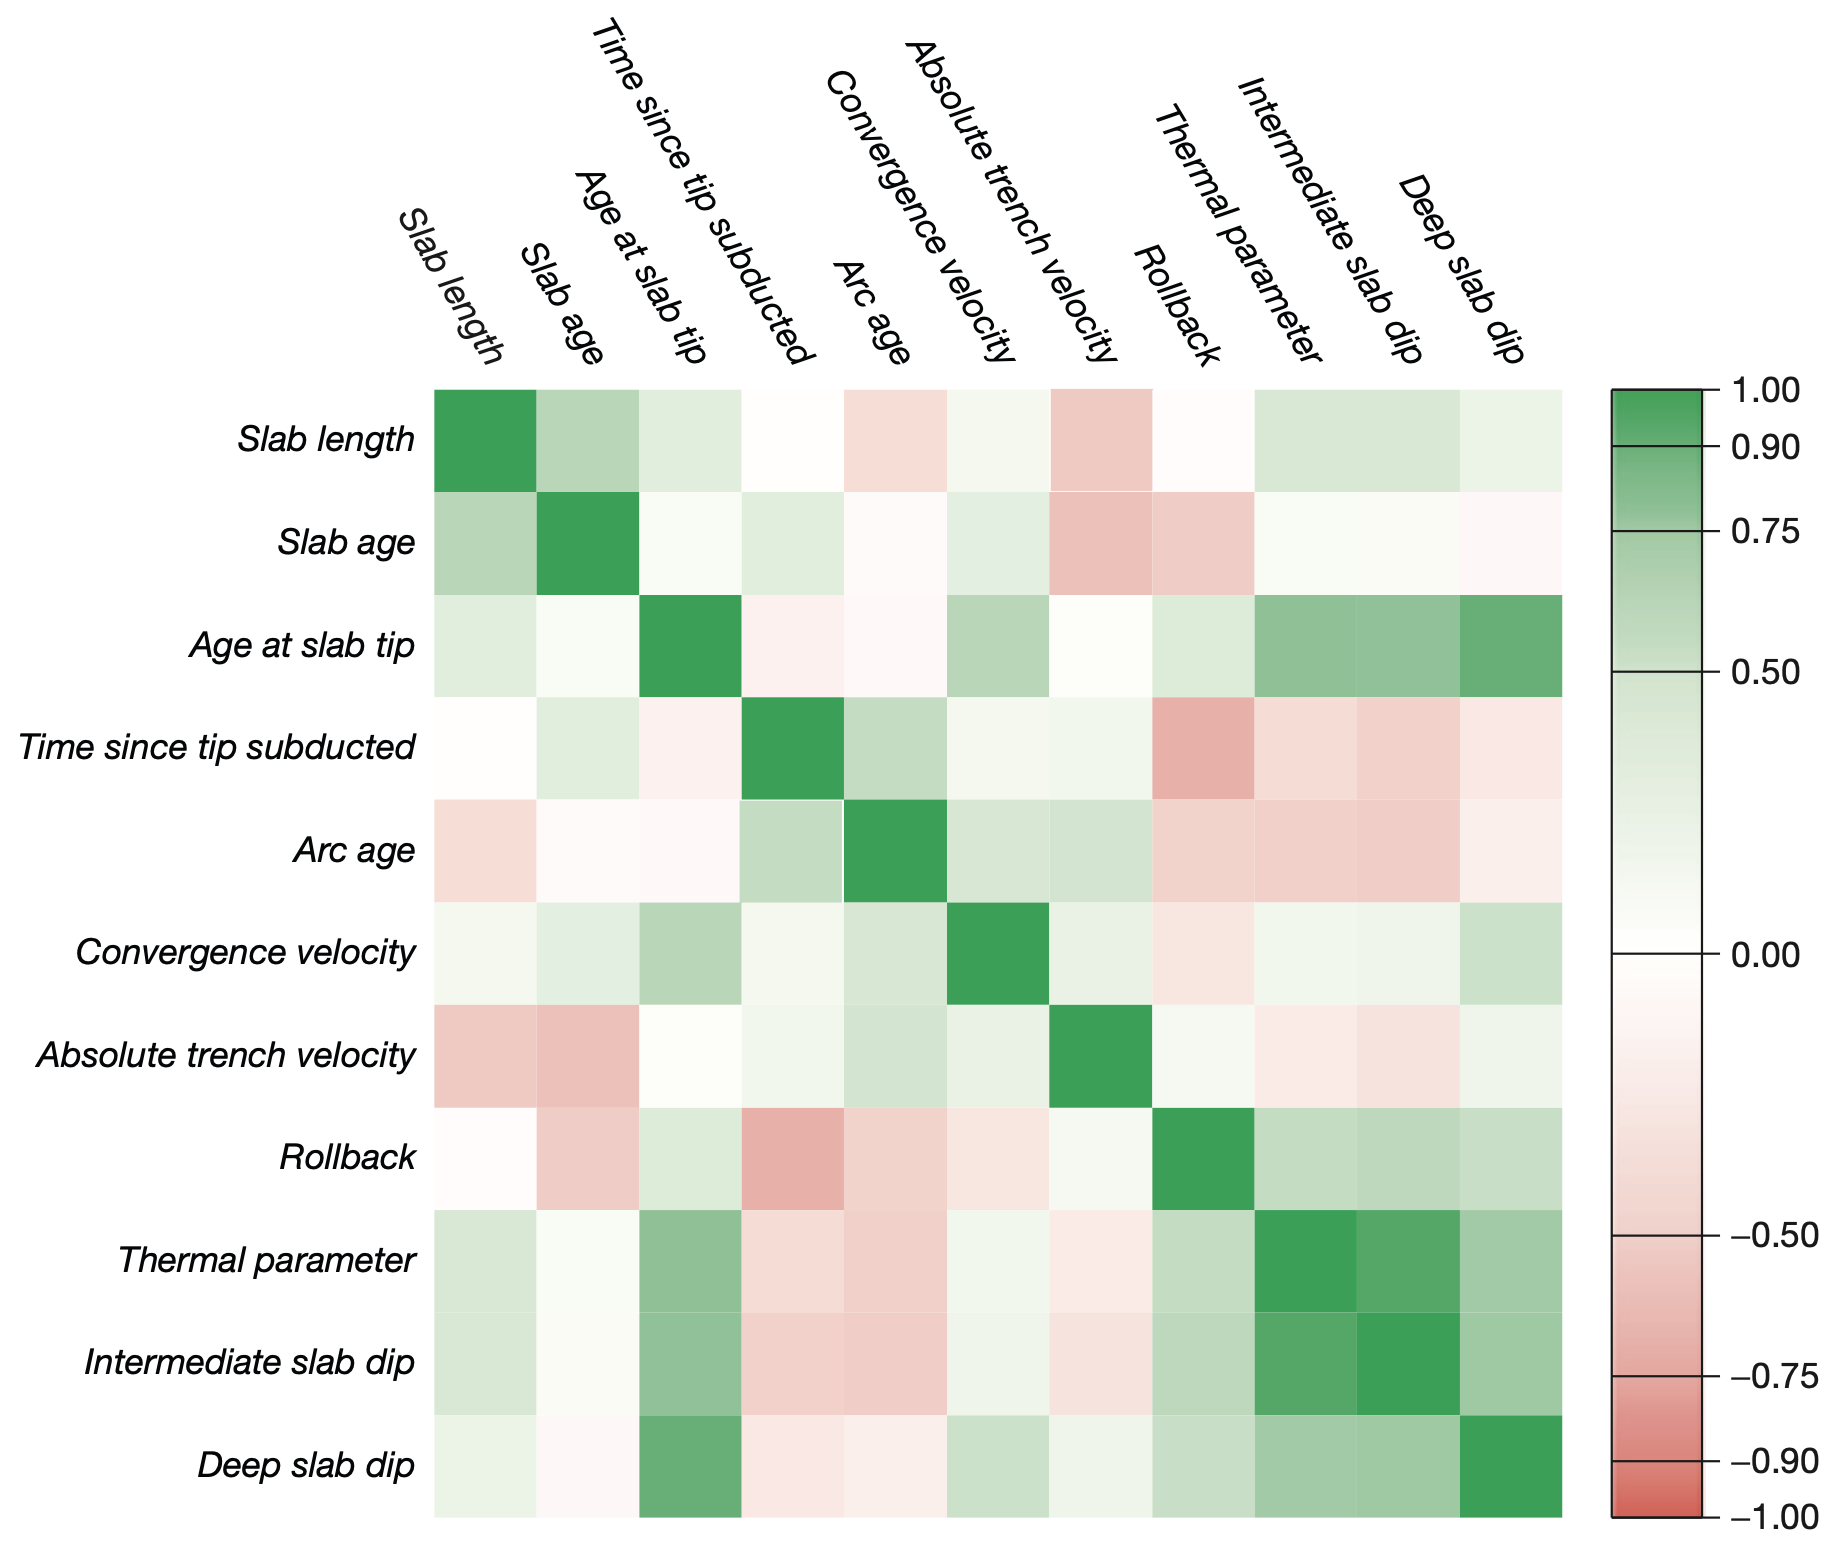
\includegraphics[width=0.8 \columnwidth]{fig/covariance.png}
%  	\caption{\label{covariance}Matriz de correlação para 9 características de 39 zonas de subducção. O valor +1.0 representa forte correlação e o valor -1.0 representa forte anticorrelação. Adaptado de \cite{treatise7.09}.}
%  \end{center}
%\end{figure}

%Inicialmente, pretende-se utilizar uma geometria simples, tal como a da figura \ref{ridge-subduction} e as velocidades serão definidas seguindo os passos das simulações de \cite{assuncao2019}, onde a subducção se desenvolve livremente a partir do peso da placa e qualquer velocidade imposta será definida em relação ao referencial de \textit{hotspots}.

%\section{Estrutura térmica}
%\label{estrutura-termica}

%A estrutura térmica inicial para o modelo sintético será uma semelhante à utilizada por \cite{assuncao2019}. Para as litosferas oceânica e continental, a temperatura aumentará linearmente com a profundidade, mas será considerada uma produção de calor radiogênico para a última. O limite entre a litosfera e a astenosfera (LAB) corresponderá à isoterma de 1300ºC.

%Para o manto, a temperatura será considerada uniforme exceto pela componente adiabática, dada pela equação \ref{adiabatic_curve} \citep{stein2009introduction}.
%\begin{equation}{\label{adiabatic_curve}}
	%T(z)=(T_0-273.15)\exp{\frac{\alpha g z}{C_p}}
%\end{equation}

%\noindent onde $T_0$ é a temperatura potencial do manto na superfície. A equação \ref{adiabatic_curve} precisa ser resolvida para $T_0$ pois a temperatura na base do modelo será fixada e definida de acordo com a reologia adotada, que será função da temperatura e do fator composicional.

%A figura \ref{thermal-structure} mostra uma estrutura térmica para uma placa em subducção e como as fácies metamórficas mudam com o aumento da profundidade e da temperatura. A configuração térmica apresentada na figura \ref{thermal-structure} corresponde, aproximadamente, à trajetória normal na figura \ref{subduction-path}.

%\begin{figure}[htb]
 % \begin{center}
  %  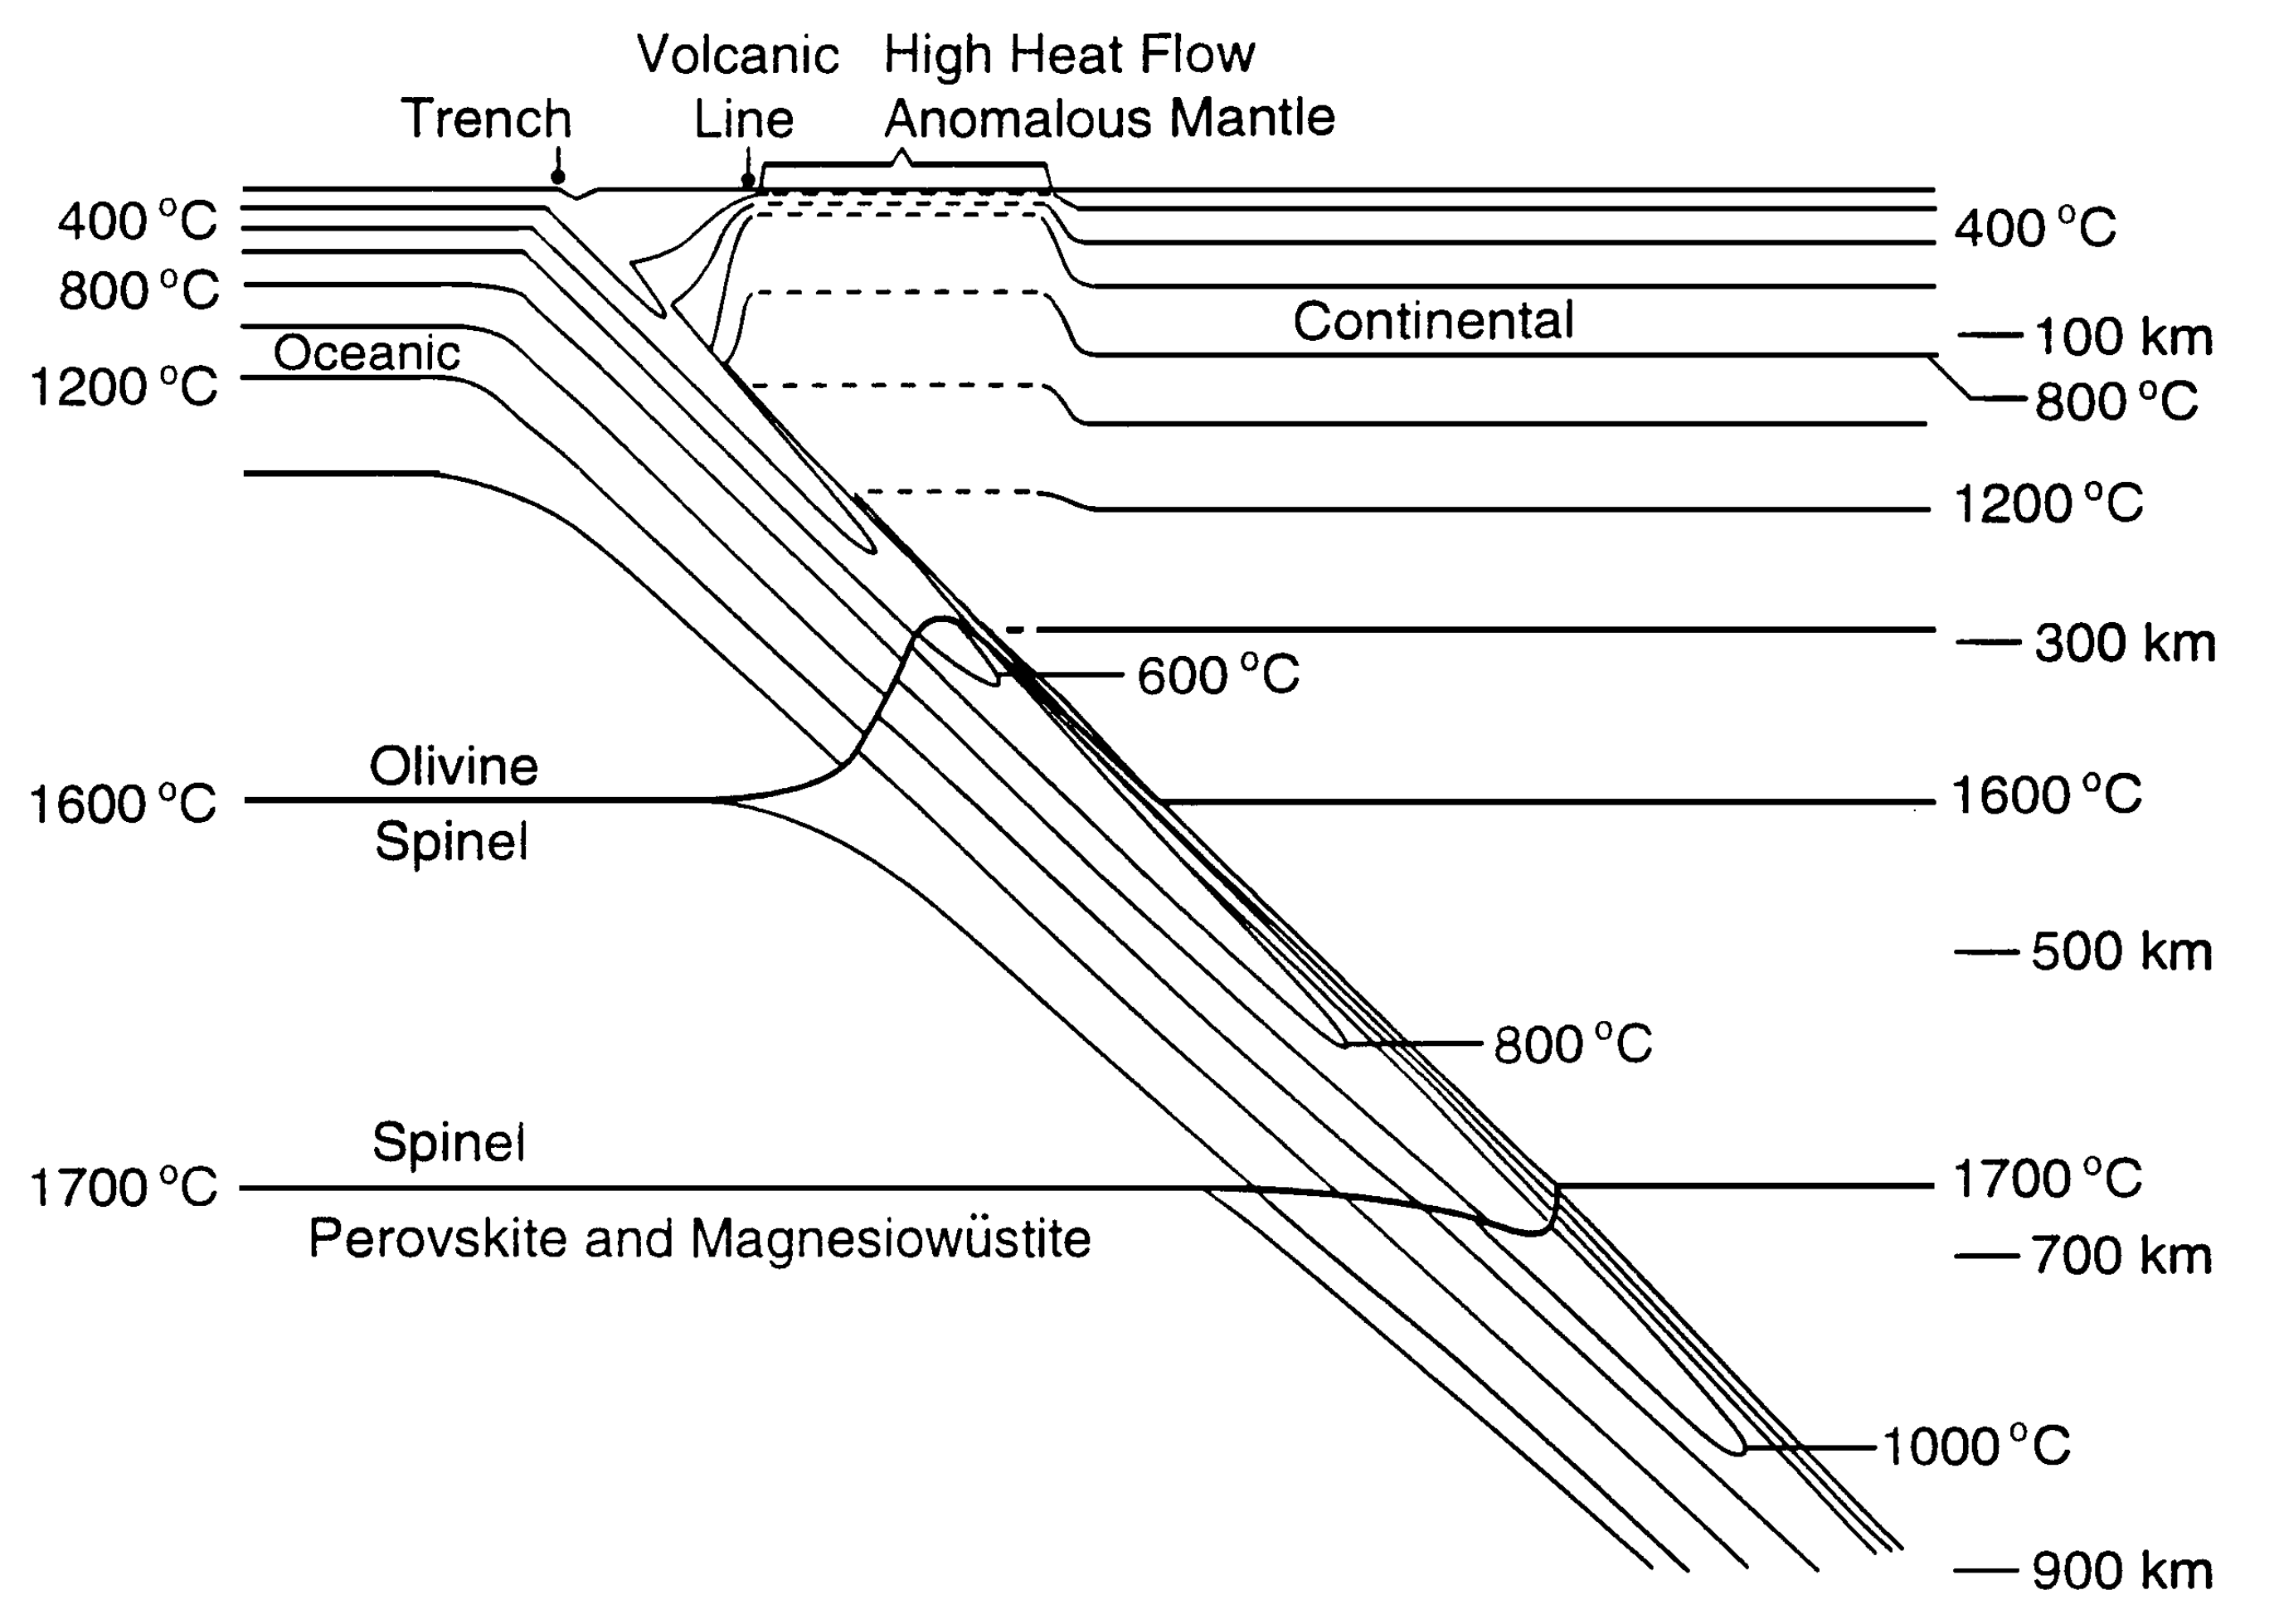
\includegraphics[width=0.8 \columnwidth]{fig/thermal-structure.png}
  %	\caption{\label{thermal-structure}Estrutura térmica de uma placa em subducção. Retirado de \cite{turcotte2002geodynamics}.}
  %\end{center}
%\end{figure}

%Outros modelos também serão explorados para definir o campo de temperatura dentro da placa em subducção, como aqueles utilizados por \cite{stein2009introduction} e \cite{minear1970thermal}.


